%\chapter{Budgeted \gls{RL} in Continuous State Space}
\chapter{The Dialogue Manager as a safe policy }
\label{chapter:nips}

In this chapter and in \Cref{chapter:slsp}, we formulate the hypothesis that the first \idx{dialogue}s with a new \idx{user} should be handled in a conservative way, for two reasons: to avoid \idx{user} dropout; and to ensure the gathering of informative \idx{dialogue}s to speedup the learning. We propose to design and transfer a  generic safe policy\index{safe policy} to handle the early interactions with the target user. The transfering algorithm is developped in \Cref{chapter:slsp}, but first, we study here how to compute this policy\index{safe policy}. Therefore, we cast the \idx{dialogue} problem as a \acrfull{BMDP} and propose a new \acrfull{RL} framework to learn safe policies\index{safe policy} in this context. A \gls{BMDP} is an extension of an \acrfull{MDP} to critical applications requiring safety constraints. It relies on a notion of risk implemented in the shape of a cost signal constrained to lie below an -- adjustable -- threshold. For our application, the risk is described as a user hanging up the conversation. The threshold is then the maximum hangup frequency we can afford with a user. So far, \glspl{BMDP} could only be solved in the case of finite state spaces with known dynamics. However, as we seen earlier, dialogue policies take as input continuous variables as the \gls{SRS} and we do not know the dynamic of a human dialoguing. As a consequence, this work extends the state-of-the-art to continuous spaces \idx{environment}s and unknown dynamics. We show that the solution to a \gls{BMDP} is a fixed point of a novel Budgeted\index{budget} Bellman Optimality\index{Bellman Optimality} operator. This observation allows us to introduce natural extensions of \acrfull{DRL} algorithms to address large-scale \glspl{BMDP}. In addition to the \gls{DS} application, we validate our approach with an autonomous driving application\footnote{The work in the chapter has been done in collaboration with Edouard Leurent. I (Nicolas Carrara) handled the creation and implementation of a novel algorithm (BFTQ) and the early proofs of concept on 2D worlds. I also made the experiments on dialogue systems. Edouard Leurent and I worked togetheir on the proofs and a novel exploration procedure. Finally, Edouard Leurent handled the autonomous driving experiments.}


\section{Motivation}
\label{sec:intro}

As stated in \Cref{chapter:dm-rl}, \gls{RL} is a general framework for decision-making under uncertainty. Formally, we seek a policy $\policy\in\cM(A)^{\cS}$ that maximises in expectation the $\discountfactor$-discounted return of rewards $\return^{\policy} = \sum_{t=0}^\infty \discountfactor^t \reward(s_t, a_t)$.

However, this modelling assumption comes at a price: no control is given over the spread of the performance distribution \parencite{Dann2018}. In many critical real-world applications, including dialogue systems, failures may \idx{turn} out very costly. This is an issue as most decision-makers would rather give away some amount of expected optimality to increase the performances in the lower-tail of the distribution. This has led to the development of several risk-averse variants where the optimisation criteria include other statistics of the performance, such as the worst-case realisation \parencite{Iyengar2005,Nilim2005,Wiesemann2013}, the variance-penalised expectation \parencite{Tamar2012,Garcia2015}, the Value at Risk \parencite{Mausser2003,Luenberger2013}, or the Conditional Value at Risk \parencite{Chow2014,ChowGJP15}.

\acrlong{RL} also assumes that the performance can be described by a single reward function $\reward$. Conversely, real problems typically involve many aspects, some of which can be contradictory \parencite{Liu2014}. For instance, a self-driving car needs to balance between progressing quickly on the road and avoiding collisions. When aggregating several objectives in a single scalar signal, as often in Multi-Objectives Reinforcement Learning~\parencite{Roijers2013ASO}, no control is given over their relative ratios, as high rewards can compensate high penalties. For instance, if a weighted sum is used to balance velocity $v$ and crashes $c$, then for any given choice of weights $\omega$ the optimality equation $\omega_v\expectedvalue[\sum\discountfactor^t v_t] + \omega_a\expectedvalue[\sum\discountfactor^t c_t] = \return^* = \max_{\policy} \return^{\policy}$ is the equation of a line in $(\expectedvalue[\sum\discountfactor^t v_t], \expectedvalue[\sum\discountfactor^t c_t])$, and the automotive company cannot control where its optimal policy $\optimalpolicy$ lies on that line. This phenomena also occurs in dialogue systems. Let's consider a dialogue system that does not say Hello at the beginning of the dialogue; it increases the dialogue efficiency (as the task is completed faster) but impacts the dialogue quality, and may induce more users hanging up and definitive dropouts. Then, with new users, it would be preferable to say Hello while a straight to the point strategy would be more appropriate with recurrent users.

Both of these concerns can be addressed in the \gls{CMDP} setting \parencite{BEUTLER1985236,Altman95constrainedmarkov}. In this multi-objective formulation, task completion and safety are considered separately. We equip the \gls{MDP} with a cost signal $\constraint \in \Real^{\cS\times \cA}$ and a cost \idx{budget} $\budget\in\Real$. Similarly to $\return^{\policy}$, we define the return of costs $\constraintreturn^{\policy} = \sum_{t=0}^\infty \discountfactor^t \constraint(s_t, a_t)$ and the new cost-constrained objective:
\begin{equation}
    \label{eq:cmdp}
    \begin{array}{lcr}
        \displaystyle \max_{\policy\in\cM(\cA)^{\cS}} \expectedvalue[\return^{\policy} | s_0=s] & \text{ s.t. } & \expectedvalue[\constraintreturn^{\policy} | s_0=s] \leq \budget
    \end{array}
\end{equation}
This constrained framework allows for better control of the performance-safety trade-off. However, it suffers from a major limitation: the \idx{budget} has to be chosen before training, and cannot be changed afterwards.

To address this concern, the \gls{BMDP} was introduced in \parencite{Boutilier_Lu:uai16} as an extension of \glspl{CMDP} to enable the online control over the \idx{budget} $\budget$ within an interval $\budgetspace \subset \Real$ of admissible budgets\index{budget}. Instead of fixing the \idx{budget} prior to training, the objective is now to find a generic optimal policy $\optimalpolicy$ that takes $\budget$ as input so as to solve the corresponding \gls{CMDP} (Eq. \eqref{eq:cmdp}) for all $\budget\in\budgetspace$. This gives the system designer the ability to move the optimal policy $\optimalpolicy$ in real-time along the Pareto-optimal curve of the different reward-cost trade-offs.

\subsection{A remark on deterministic policies}
%
A convenient property of \glspl{MDP}, is that the optimal policy is unique, deterministic\index{deterministic policy} and \idx{greedy}: $\optimalpolicy(s)=\argmax_{a}\Q(s,a)$.
In a \gls{CMDP}, and \textit{a fortiori} in a \gls{BMDP}, this is in general not the case. It has been shown indeed that the optimal policy under constraint is a random mixture of two deterministic policies\index{deterministic policy} \textcite[Theorem 4.4]{BEUTLER1985236}.

To illustrate this fact, let us consider the trivial \gls{BMDP} on the left of \Cref{fig:stochasticneeded}.
On this example we have $\return^{\policy}=10\pi_1$ and $\constraintreturn^{\policy}=\pi_1$. The \idx{deterministic policy} consisting in always picking the safe action is feasible for any $\budget\geq 0$. But if $\budget=1/2$, the most rewarding feasible policy is to randomly pick the safe and risky actions with equal probabilities.
If we attempt to cast this \gls{BMDP} into an MDP by replacing the costs by negative rewards, the policy we will obtain will be deterministic\index{deterministic policy}, hence sub-optimal.
%
\begin{figure}
    \centering
    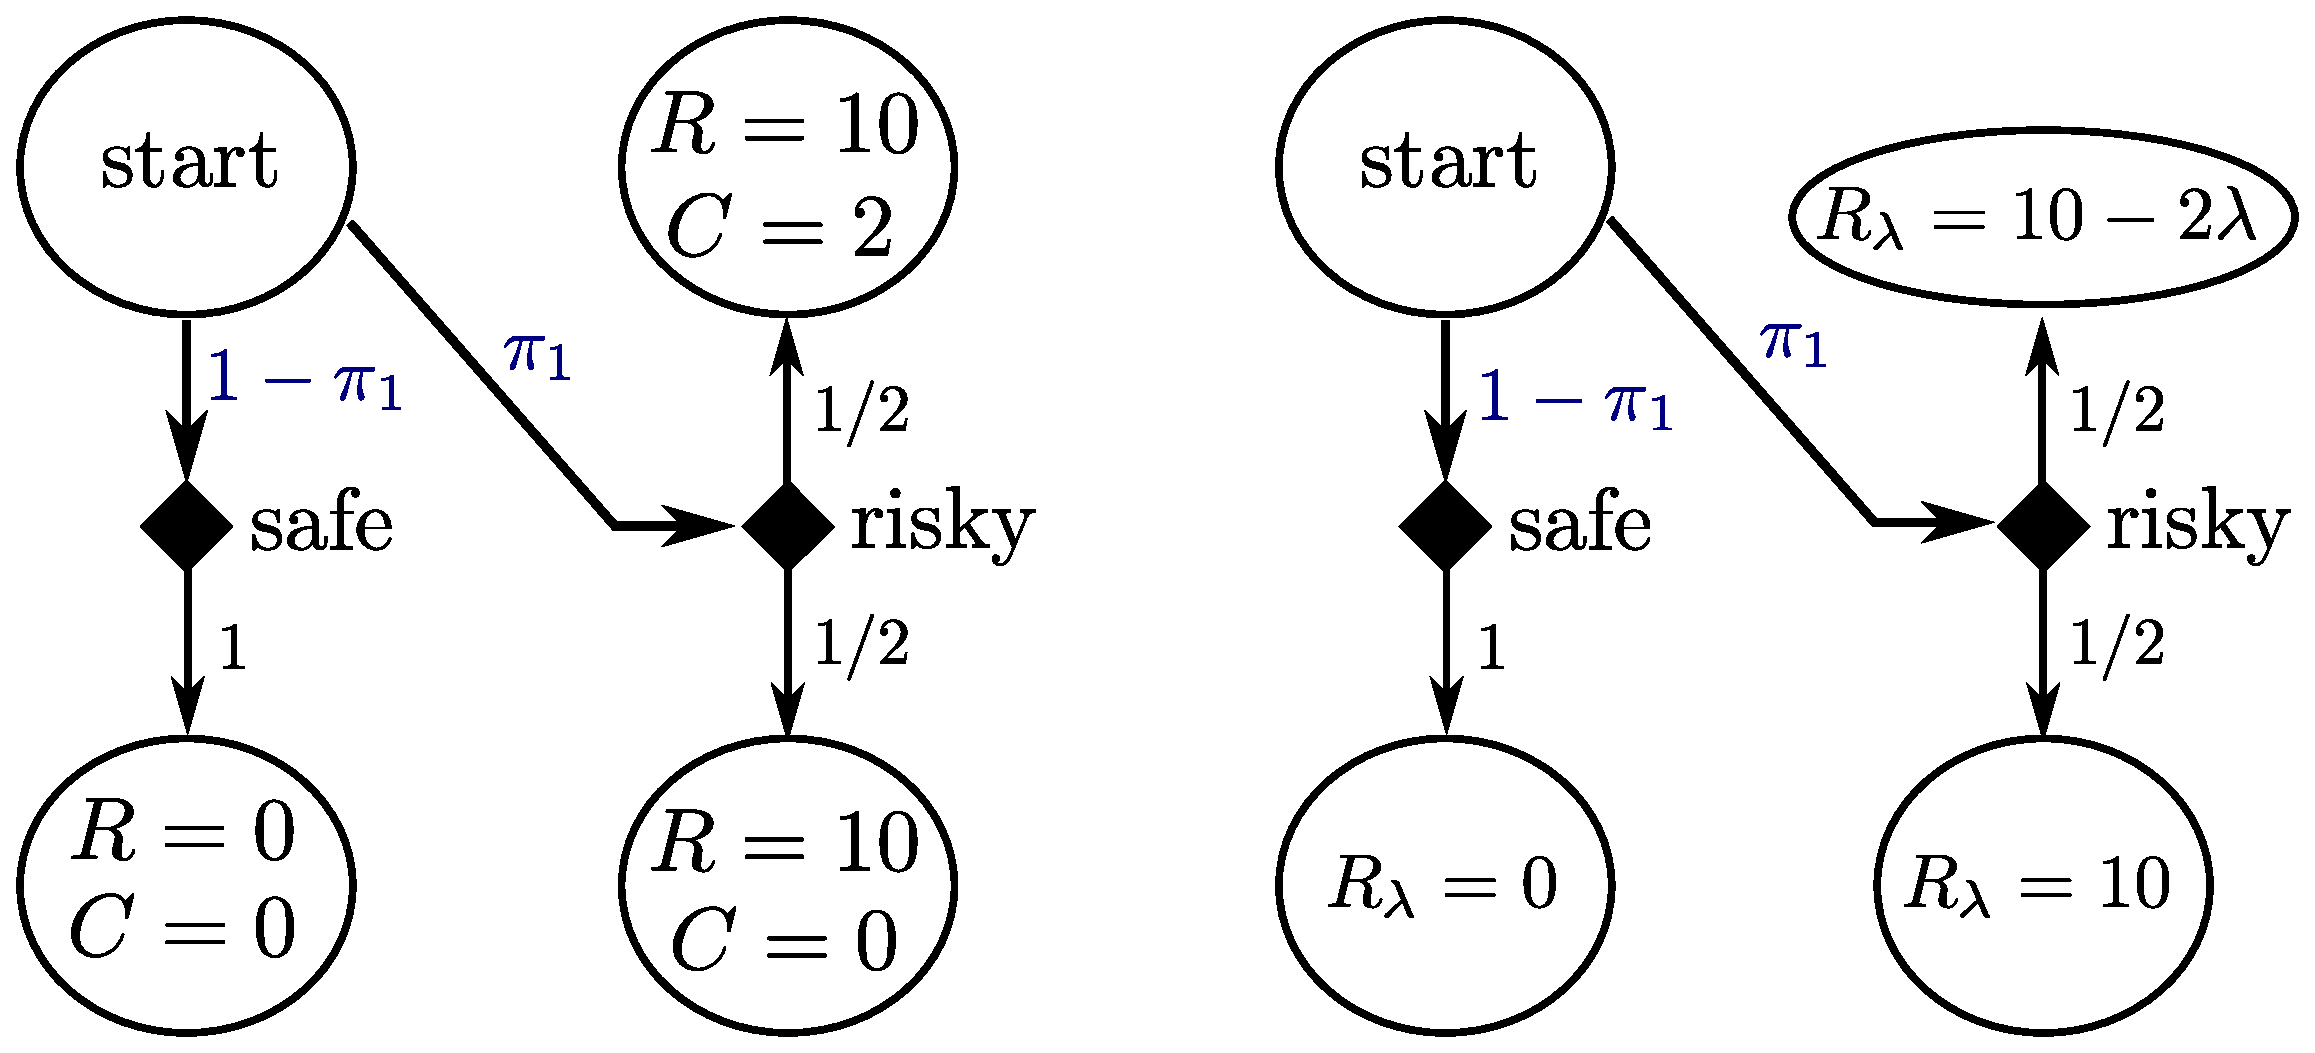
\includegraphics[width=0.6\textwidth]{sources/contribution/nips/source/img/SafeRiskyExample}
    \caption[Example of relaxed Budgeted Markov Decision Process]{On the left hand side, a simple \textit{risky-vs-safe} \gls{BMDP}. The probability of picking the risky action is $\pi_1$. On the right hand side an attempt to relax the problem with negative rewards.}
    \label{fig:stochasticneeded}
\end{figure}

Our first contribution is to re-frame the original \gls{BMDP} formulation in the context of continuous states and infinite discounted horizon. We then propose a novel Budgeted\index{budget} Bellman Optimality\index{Bellman Optimality} Operator and prove the optimal value function to be a fixed point of this operator. Second, we use this operator in \gls{BFTQ}, a \idx{batch} \gls{RL} algorithm, for solving \glspl{BMDP} \idx{Online} by interacting with an \idx{environment}, through function approximation and a tailored exploration procedure. Third, we scale this algorithm to large problems by providing an efficient implementation of the Budgeted\index{budget} Bellman Optimality\index{Bellman Optimality} operator based on convex programming, and by leveraging tools from \gls{DRL} such as \glspl{NN} and synchronous parallel computing. Finally, we validate our approach in two \idx{environment}s that display a clear trade-off between rewards and costs: a \gls{SDS} and a problem of behaviour planning for autonomous driving. The proofs of our main results are provided \Cref{sec:proofs}.

\section{Budgeted Dialogue Policies}
\label{sec:bdp}
We work in the space of budgeted policies\index{budgeted policy}, where $\policy$ both depends on $\budget$ and also outputs a next \idx{budget} $\budgetaction$. Hence, the \idx{budget} $\budget$ is neither fixed nor constant as in the \gls{CMDP} setting but instead evolves as part of the dynamics.

We cast the \gls{BMDP} problem as a multi-objective MDP problem \parencite{Roijers2013ASO} by considering \emph{augmented} state and action spaces $\ocS = \cS\times \budgetspace$ and $\ocA= \cA\times \budgetspace$, and equip them with the augmented dynamics $\augmentedtransition\in \cM(\ocS)^{\ocS \times \ocA}$ defined as:
\begin{equation}
    \label{eq:dynamics}
    \augmentedtransition\left(\os' \condbar \os, \oa\right) = \augmentedtransition\left((s',\nextbudget) \condbar (s,\budget), (a, \budgetaction)\right) \eqdef \transition(s'|s, a)\dirac(\nextbudget - \budgetaction),
\end{equation}
where $\dirac$ is the Dirac indicator distribution.

In other words, in these augmented dynamics, the output \idx{budget} $\budgetaction$ returned at time $t$ by a \idx{budgeted policy} $\budgetedpolicy\in \policies=\cM(\ocA)^{\ocS}$ will be used to condition the policy at the next timestep $t+1$.

We stack the rewards and cost functions in a single \emph{vectorial} signal $\augmentedreward \in (\Real^2)^{{\ocS \times \ocA}}$:

\begin{definition}
    Given an augmented \idx{transition} $(\os, \oa) =((s,\budget), (a, \budgetaction))$, we define:
    \begin{equation}
    \augmentedreward(\os, \oa) \eqdef  \begin{bmatrix}
                              \reward(s, a)\\
                              \constraint(s, a)
    \end{bmatrix}\in\Real^2.
\end{equation}
\end{definition}

Likewise, we augment the return:

\begin{definition}
    The return $\augmentedreturn^{\budgetedpolicy} = (\return^{\budgetedpolicy}, \constraintreturn^{\budgetedpolicy})$ of a \idx{budgeted policy} $\budgetedpolicy\in\policies$ refers to:
    \begin{equation}
        \augmentedreturn^{\budgetedpolicy} \eqdef \sum_{t=0}^\infty \discountfactor^t \augmentedreward(\os_t, \oa_t).
    \end{equation}
\end{definition}

We also augment the value functions:

\begin{definition}
    The value functions $\oV^{\budgetedpolicy}$, $\oQ^{\budgetedpolicy}$ of a \idx{budgeted policy} $\budgetedpolicy\in\policies$ are defined as:
    \begin{equation}
        \label{eq:value-function}
        \oV^{\budgetedpolicy}(\os) = (\Vr^{\budgetedpolicy}, \Vc^{\budgetedpolicy}) \eqdef \expectedvalue\left[ \augmentedreturn^{\budgetedpolicy} \condbar \ov{s_0} = \os\right] \\
        \oQ^{\budgetedpolicy}(\os, \oa)= (\Qr^{\budgetedpolicy}, \Qc^{\budgetedpolicy}) \eqdef \expectedvalue\left[ \augmentedreturn^{\budgetedpolicy} \condbar \ov{s_0} = \os, \ov{a_0} = \oa\right].
    \end{equation}
\end{definition}

We restrict $\ocS$ to feasible budgets\index{budget} only: $\ocS_f \eqdef \{(s,\budget)\in\ocS: \exists \budgetedpolicy\in\policies, \Vc^{\budgetedpolicy}(s) \leq \budget\}$ that we assume is non-empty for the \gls{BMDP} to admit a solution. We still write $\ocS$ in place of $\ocS_f$ for brevity of notations.

\begin{proposition}[Budgeted\index{budget} Bellman Evaluation\index{Bellman Evaluation}]
    \label{prop:bellman-expectation}
    The value functions $\oV^{\budgetedpolicy}$ and $ \oQ^{\budgetedpolicy}$ verify:
    \begin{align}
        \oV^{\budgetedpolicy}(\os) = \sum_{\oa\in\ocA}\budgetedpolicy(\oa | \os) \oQ^{\budgetedpolicy}(\os, \oa) \qquad \oQ^{\budgetedpolicy}(\os, \oa) = \gls{oR}(\os, \oa) + \discountfactor\sum_{\os'\in\ocS}\augmentedtransition\left(\os' \condbar \os, \oa\right) \oV^{\budgetedpolicy}(\os'). \label{eq:bellman_expectation}
    \end{align}
    Moreover, consider the Budgeted\index{budget} Bellman Evaluation\index{Bellman Evaluation} operator $\abo^{\budgetedpolicy}$:
    $\forall \oQ\in(\Real^2)^{\ocS\ocA}, \os\in\ocS, \oa\in\ocA$,
    \begin{align}
        \label{eq:bellman_expectation_operator}
        \abo^{\budgetedpolicy} \oQ(\os, \oa) &\eqdef \gls{oR}(\os, \oa) + \discountfactor \sum_{\os'\in\ocS}\sum_{\oa'\in\ocA}\augmentedtransition(\os'|\os, \oa)\budgetedpolicy(\oa'|\os') \oQ(\os', \oa').
    \end{align}
    Then $\abo^{\budgetedpolicy}$ is a $\discountfactor$-contraction and $\oQ^{\budgetedpolicy}$ is its unique fixed point.
\end{proposition}

\begin{proof}
    The proof is available in \Cref{proof-bellman-expectation}
\end{proof}

\begin{definition}[Budgeted Optimality]
    We now come to the definition of budgeted optimality. We want an optimal \idx{budgeted policy} to: (i)~respect the cost budget $\budget$, (ii)~maximise the $\discountfactor$-discounted return of rewards $\return$, (iii)~in case of tie, minimise the $\discountfactor$-discounted return of costs $\constraintreturn$. To that end, we define for all $\os\in\ocS$:
    \begin{enumerate}[(i)]
        \item Admissible policies $\policies_a$:
        \begin{equation}
            \policies_a(\os) \eqdef \{\budgetedpolicy\in\policies: \Vc^{\budgetedpolicy}(\os) \leq \budget\}\text{ where }\os = (s, \budget)
        \end{equation}
        \item Optimal value function for rewards $\Vr^*$ and candidate policies $\policies_r$:
        \begin{equation}
            \Vr^*(\os) \eqdef \max_{\budgetedpolicy\in\policies_a(\os)}  \Vr^{\budgetedpolicy}(\os) \qquad\qquad \policies_r(\os) \eqdef \argmax_{\budgetedpolicy\in\policies_a(\os)}  \Vr^{\budgetedpolicy}(\os)
        \end{equation}
        \item Optimal value function for costs $\Vc^*$ and optimal policies $\policies^*$:
        \begin{equation}
            \Vc^*(\os) \eqdef \min_{\budgetedpolicy\in\policies_r(\os)}  \Vc^{\budgetedpolicy}(\os), \qquad\qquad \policies^*(\os) \eqdef \argmin_{\budgetedpolicy\in\policies_r(\os)}  \Vc^{\budgetedpolicy}(\os)
        \end{equation}
    \end{enumerate}
    We define the budgeted action-value function $\oQ^*$ similarly:
    \begin{equation}
        \Qr^*(\os, \oa) \eqdef \max_{\budgetedpolicy\in\policies_a(\os)}  \Qr^{\budgetedpolicy}(\os, \oa) \qquad\qquad \Qc^*(\os, \oa) \eqdef \min_{\budgetedpolicy\in\policies_r(\os)}  \Qc^{\budgetedpolicy}(\os, \oa)
    \end{equation}
    and denote $\oV^* = (\Vr^*, \Vc^*)$, $\oQ^* = (\Qr^*, \Qc^*)$.
\end{definition}

\begin{theorem}[Budgeted Bellman Optimality]
    \label{thm:bellman-optimality}
    The optimal budgeted action-value function $\oQ^*$ verifies:
    \begin{equation}
        \label{eq:bellman-optimality}
        \oQ^{*}(\os, \oa) = \abo^{*}\oQ^{*}(\os, \oa) \eqdef \gls{oR}(\os, \oa) + \discountfactor \sum_{\os'\in\ocS} \augmentedtransition(\ov{s'} | \os, \oa)\sum_{\ov{a'}\in \ocA} \budgetedpolicy_\text{greedy}(\ov{a'}|\ov{s'}; \oQ^*) \oQ^{*}(\ov{s'}, \ov{a'}),
    \end{equation}
    where the \idx{greedy} policy $\budgetedpolicy_\text{greedy}$ is defined by: $\forall \os=(s,\budget)\in \ocS, \oa\in
    \ocA, \forall \oQ\in(\Real^2)^{\ocA\times\ocS},$
    \begin{subequations}
        \label{eq:pi_greedy}
        \begin{align}
            \budgetedpolicy_\text{greedy}(\oa|\os; \oQ) \in &\argmin_{\rho\in\policies_r^{\oQ}} \expectedvalueover{\oa\sim\rho}\Qc(\os, \oa), \label{eq:pi_greedy_cost}\\
            \text{where }\quad\policies_r^{\oQ} \eqdef &\argmax_{\rho\in\cM(\ocA)} \expectedvalueover{\oa\sim\rho} \Qr(\os, \oa) \label{eq:pi_greedy_reward}\\
            & \text{ s.t. }  \expectedvalueover{\oa\sim\rho} \Qc(\os, \oa) \leq \budget. \label{eq:pi_greedy_constraint}
        \end{align}
    \end{subequations}
\end{theorem}

\begin{proof}
    The proof is available in \Cref{proof-thm:bellman-optimality}
\end{proof}

\begin{remark}[Appearance of the \idx{greedy} policy]
    \label{rmk:greedy}
    In classical \gls{RL}, the \idx{greedy} policy takes a simple form $\policy_\text{greedy}(s; \Q^*) = \argmax_{a\in\cA} \Q^*(s, a)$, and the term $\policy_\text{greedy}(a'|s';\Q^*) \Q^{*}(s', a')$ in \eqref{eq:bellman-optimality} conveniently simplifies to $\max_{a'\in \cA} \Q^*(s', a')$. Unfortunately, in a budgeted setting the \idx{greedy} policy requires solving the nested constrained optimisation program \eqref{eq:pi_greedy} at each state and budget in order to apply this Budgeted Bellman Optimality operator.
\end{remark}

\begin{proposition}[Optimality of the \idx{greedy} policy]
    \label{prop:greedy_optimal}
    The \idx{greedy} policy $\budgetedpolicy_\text{greedy}(\cdot~; \oQ^*)$ is \emph{uniformly} optimal: for all $\os\in\ocS$, $\budgetedpolicy_\text{greedy}(\cdot~; \oQ^*)\in\policies^*(\os)$. In particular, $\oV^{\budgetedpolicy_\text{greedy}(\cdot; \oQ^*)} = \oV^*$ and $\oQ^{\budgetedpolicy_\text{greedy}(\cdot; \oQ^*)}= \oQ^*$.
\end{proposition}

\begin{proof}
    The proof is available in \Cref{proof-prop:greedy_optimal}
\end{proof}

\begin{theorem}[Contractivity of $\abo^{*}$]
    \label{thm:contraction}
    For any \gls{BMDP} ($\cS,\cA,\transition,\reward,\constraint,\discountfactor$) with $|\cA| \geq 2$, $\abo^{*}$ is not a contraction.
\end{theorem}

\begin{proof}
    The proof is available in \Cref{proof-thm:contraction}
\end{proof}

\paragraph{Budgeted Value Iteration}


The Budgeted Bellman Optimality equation is a fixed-point equation, which motivates the introduction of a fixed-point iteration procedure. We introduce \Cref{algo:bvi}, a Dynamic Programming algorithm for solving known \glspl{BMDP}.

\begin{algorithm}
    \DontPrintSemicolon
    \KwData{$\transition, \reward, \constraint$}
    \KwResult{$\oQ^*$}
    $\oQ_{0} \leftarrow 0$\;
    \Repeat{convergence}{
    $\oQ_{k+1} \leftarrow \abo^{*}\oQ_k$\;
    }
    \caption{Budgeted Value-Iteration}
    \label{algo:bvi}

\end{algorithm}

Unfortunately, as $\abo^{*}$ is not a contraction, we can guarantee neither the convergence of this procedure nor the unicity of its fixed points. Despite those theoretical limitations, we empirically observed the convergence to a fixed point in our experiments (\Cref{sec:experiements}). We conjecture a possible explanation:

\begin{theorem}[Contractivity of $\abo^{*}$ on smooth $\oQ$-functions]
    \label{thm:contractivity-smooth}
    The operator $\abo^{*}$ is a contraction when restricted to the subset $\cL_{\discountfactor}$ of $\oQ$-functions such that "$\Qr$ is $L$-Lipschitz with respect to $\Qc$", with $L<\frac{1}{\discountfactor}-1$.
\end{theorem}

\begin{proof}
    The proof is available in \Cref{proof-contraction-with-smooth}
\end{proof}

\section{Budgeted Reinforcement Learning}
\label{sec:brl}

In this section, we consider \glspl{BMDP} with unknown parameters that must be solved by interaction with an \idx{environment}.

\subsection{Budgeted Fitted-$Q$}
\label{subsec:bftq}

When the \gls{BMDP} is unknown, we need to adapt \Cref{algo:bvi} to work with a \idx{batch} of \idx{transition}s $\cD=\{(\os_{\indextransition},\oa_{\indextransition},\overline{r}_{\indextransition},\os_{\indextransition}'\}_{{\indextransition}\in [0,N]}$ collected by interaction with the \idx{environment}. Applying $\abo^{*}$ in \eqref{eq:bellman-optimality} would require computing an expectation $\expectedvalue_{\os'\sim \augmentedtransition}$ over next states $\os'$ and hence an access to the \idx{model} $\augmentedtransition$. We instead use $\hat{\abo^{*}}$, a sampling operator, in which this expectation is replaced by:
\begin{equation*}
    \hat{\abo^{*}} \oQ(\os_{\indextransition}, \oa_{\indextransition}, \overline{r}_{\indextransition}, \os'_{\indextransition}) \eqdef \overline{r}_{\indextransition} + \discountfactor \sum_{\ov{a'_{\indextransition}}\in \ov{\cA}} \budgetedpolicy_\text{greedy}(\ov{a'_{\indextransition}}|\ov{s'_{\indextransition}}; \oQ) \oQ(\ov{s'_{\indextransition}}, \ov{a'_{\indextransition}}).
\end{equation*}
We introduce in \Cref{algo:bftq} the \gls{BFTQ} algorithm, an extension of the \gls{FTQ} algorithm adapted to solve unknown \glspl{BMDP}. Because we work with continuous state space $\cS$ and budget space $\budgetspace$, we need to employ function-approximation in order to generalise to nearby states and budgets. Following the same idea used in \gls{FVI}, we introduce a projection operator $\augmentedprojection$ onto $\ocF$, the set of representable functions with domain $\ocS\times\ocA$ into $\Real^2$: $\augmentedprojection f = \argmin_{\tilde{f}\in \ocF} || f - \tilde{f} ||_{\infty}$. \gls{BFTQ} simply iterates over the following equation: $\oQ_{k+1} \leftarrow \augmentedprojection\hat{\abo^{*}} \oQ_k$.

To operate the projection we choose a least-square \idx{regression} algorithm. Precisely, given a parametrised \idx{model} $\oQ_{\params}$, we seek to minimise a \idx{regression} loss $\cL(\oQ_{\params}, \oQ_\text{target};\cD) = \sum_{\cD} ||\oQ_{\params}(\os, \oa) - \oQ_\text{target}(\os, \oa, \overline{r}, \os')||_2^2$. Any \idx{model} can be used, such as linear models\index{linear model}, \idx{regression} trees, or neural networks.

\begin{algorithm}[H]
    \DontPrintSemicolon
    \KwData{$\cD$}
    \KwResult{$\oQ^*$}
    $\oQ_{0} \leftarrow 0$\;
    \Repeat{convergence}{
    $\params_{k+1} \leftarrow \argmin_{\params} \cL(\oQ_{\params}, \hat{\abo^{*}} \oQ_{\params_{k}}; \cD)$\;
    }
    \caption{Budgeted Fitted-$Q$}
    \label{algo:bftq}

\end{algorithm}

\subsection{Risk-sensitive exploration}
\label{sec:exploration}

In order to run \Cref{algo:bftq}, we must first gather a \idx{batch} of \idx{transition}s $\cD$. Ideally we would need \idx{transition}s from the asymptotic state-budget distribution $\lim_{t\rightarrow\infty}\probability{\os_t}$ induced by an optimal policy $\optimalbudgetedpolicy$ given an initial distribution $\probability{\os_0}$, but as we are actually building this policy, it is not possible. Following the same idea of \idx{$\egreedy$-greedy} exploration for \gls{FTQ}, we introduce an algorithm for \idx{risk-sensitive} exploration. We follow an exploration policy: a mixture between a random \idx{budgeted policy} $\budgetedpolicy_\text{rand}$ and the current \idx{greedy} policy $\budgetedpolicy_\text{greedy}$. The \idx{batch} $\cD$ is split into several minibatches\index{batch} generated sequentially, and $\budgetedpolicy_\text{greedy}$ is updated by running \Cref{algo:bftq} on $\cD$ upon mini-batch\index{batch} completion. $\budgetedpolicy_\text{rand}$ is designed to obtain trajectories\index{trajectory} that only explore feasible budgets: we impose that the joint distribution $\probability{a, \budgetaction|s, \budget}$ verifies $\expectedvalue[\budgetaction]\leq\budget$. This condition defines a probability simplex $\Delta_{\ocA}$ from which we \idx{transition} uniformly. Finally, when interacting with an \idx{environment} the initial state $s_0$ is usually sampled from a starting distribution $\probability{s_0}$. In the budgeted setting, we also need to \idx{transition} the initial budget $\budget_0$. Importantly, we pick a uniform distribution $\probability{\budget_0} = \cU(\budgetspace)$ so that the entire range of risk-level is explored, and not only reward-seeking behaviours as would be the case with a traditional \idx{risk-neutral} \idx{$\egreedy$-greedy} strategy. The pseudo-code of our exploration procedure is shown in \Cref{algo:risk-sensitive-exploration}.

\begin{algorithm}[ht!]
\DontPrintSemicolon
\KwData{An \idx{environment}, a \gls{BFTQ} solver, $W$ \gls{CPU} workers}
\KwResult{A \idx{batch} of \idx{transition}s $\cD$}
$\cD\leftarrow\{\}$\;
\For{each intermediate \idx{batch}} {
split trajectories\index{trajectory} between $W$ workers\;
\For(\tcp*[f]{run this loop on each worker in parallel}){each trajectory\index{trajectory} in \idx{batch}}{
sample initial budget $\budget\sim\cU(\binomial(1,B)$.\;
\While{trajectory\index{trajectory} not done}{
update $\egreedy$ from schedule.\;
sample $z\sim\cU([0, 1])$.\;
\lIf{$z < \egreedy$}{sample $(a, \budgetaction)\sim\cU(\Delta_{\cA\times\budgetspace})$.\tcp*[f]{Explore}}
\lElse{sample $(a, \budgetaction)\sim\budgetedpolicy_\text{greedy}(a, \budgetaction|s, \budget; \oQ^*)$.\tcp*[f]{Exploit}}
append \idx{transition} $(\os=(s, \budget),\oa=(a, \budgetaction),\overline{r}=(r, c),\os'=(s',\budgetaction))$ to \idx{batch} $\cD$.\;
step trajectory\index{trajectory} budget $\budget \leftarrow \budgetaction$
}
}
$\budgetedpolicy_\text{greedy}(\cdot\sim; ~\oQ^*) \leftarrow\texttt{BFTQ}(\cD)$.
}
\Return{the \idx{batch} of \idx{transition}s $\cD$}
\caption{Risk-sensitive exploration}
\label{algo:risk-sensitive-exploration}
\end{algorithm}


\section{A scalable Implementation}
\label{sec:scalable-bftq}
In this section, we introduce an implementation of the \gls{BFTQ} algorithm designed to operate efficiently and handle large batches\index{batch} of experiences $\cD$.

\subsection{How to compute the \idx{greedy} policy?}

\begin{figure}
    \centering
    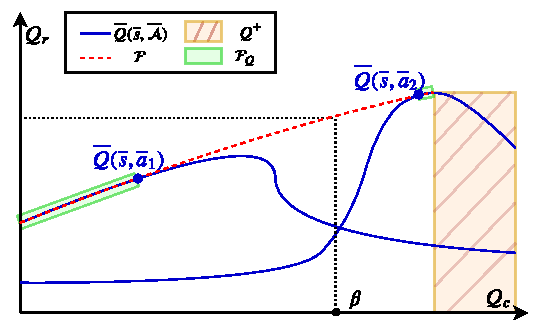
\includegraphics[width=0.75\linewidth]{sources/contribution/nips/source/img/pi.pdf}
    \caption[Representation of $\budgetedpolicy_\text{hull}$.]{Representation of $\budgetedpolicy_\text{hull}$. When the budget lies between $\oQ(\os,\oa_1)$ and $\oQ(\os,\oa_2)$, two points of the top frontier of the convex hull, then the policy is a mixture of these two points.}
    \label{fig:hull}
\end{figure}

\label{subsec:compute-greedy-policy}
As stated in \Cref{rmk:greedy}, computing the \idx{greedy} policy $\budgetedpolicy_\text{greedy}$ in \eqref{eq:bellman-optimality} is not trivial since it requires solving the nested constrained optimisation program \eqref{eq:pi_greedy}.

However, it can be solved efficiently by exploiting the \emph{structure} of the set of solutions with respect to $\budget$, that is, concave and increasing.

\begin{proposition}[Equality of $\budgetedpolicy_\text{greedy}$ and $\budgetedpolicy_\text{hull}$]
    \label{prop:bftq_pi_hull}
    \Cref{algo:bvi} and \Cref{algo:bftq} can be run by replacing $\budgetedpolicy_\text{greedy}$ in the equation \eqref{eq:bellman-optimality} of $\abo$ with $\budgetedpolicy_\text{hull}$ as described in \Cref{algo:pi_hull}.
    \begin{equation*}
        \budgetedpolicy_\text{greedy}(\oa|\os; \oQ) = \budgetedpolicy_\text{hull}(\oa|\os; \oQ)
    \end{equation*}
\end{proposition}

\begin{proof}
    The proof is available in \Cref{sec:proof_pi_hull}
\end{proof}

\begin{algorithm}
    \DontPrintSemicolon
    \KwData{$\os=(s,\budget)$, $\oQ$}
    $\oQ^+\leftarrow \{\Qc > \min \{\Qc(\os,\oa) \text{ s.t. }\oa\in\argmax_{\oa} \Qr(\os,\oa)\} \}$\tcp*[f]{dominated points}\;
    $\cF \leftarrow \text{top frontier of }\texttt{convex\_hull}(\oQ(\os,\ocA) \setminus \oQ^+)$\tcp*[f]{candidate mixtures}\;
    $\cF_{\oQ} \leftarrow \cF\cap \oQ(\os,\ocA)$\;
    \For{points $q = \oQ(\os,\oa)\in\cF_{\oQ}$ in clockwise order}{
    \uIf{find two successive points $((q_c^1, q_r^1), (q_c^2, q_r^2))$ of $\cF_{\oQ}$ such that $q_c^1 \leq \budget < q_c^2$}{
    $p \leftarrow (\budget - q_c^1) / (q_c^2 - q_c^1)$\;
    \Return the mixture $(1-p)\dirac(\oa-\oa^1) + p\dirac(\oa-\oa^2)$\;
    }}
    \lElse{\Return $\dirac(\oa - \argmax_{\oa} \Qr(\os,\oa))$\tcp*[f]{Budget $\budget$ always respected}}
    \caption{Convex hull policy $\budgetedpolicy_\text{hull}(\oa|\os; \oQ)$}
    \label{algo:pi_hull}
\end{algorithm}

The computation of $\budgetedpolicy_\text{hull}$ in \Cref{algo:pi_hull} is illustrated in \Cref{fig:hull}.

\subsection{Function approximation}

\acrlongpl{NN} are well suited to \idx{model} $\oQ$-functions in \gls{RL} algorithms \parencite{Riedmiller05,Mnih2015}. We approximate $\oQ = (\Qr, \Qc)$ using one single \gls{NN}. Thus, the two components are jointly optimised which accelerates convergence and fosters learning of useful shared representations. Moreover, as in \parencite{Mnih2015} we are dealing with a finite (categorical) action space $\cA$, instead of including the action in the input we add the output of the $\oQ$-function for each action to the last layer. Again, it provides a faster convergence toward useful shared representations and it only requires one forward pass to evaluate all action values. Finally, beside the state $s$ there is one more input to a budgeted $\oQ$-function:~the budget $\budgetaction$. This budget is a scalar value whereas the state $s$ is a vector of potentially large size. To avoid a weak influence of the budget $\budget_a$ compared to the state $s$ in the prediction, we include an additional encoder for the budget, whose width and depth may depend on the application. A straightforward choice is a single layer with the same width as the state. The overall architecture is shown in \Cref{fig:architecture}.

\begin{figure}[tp]
    \centering
    
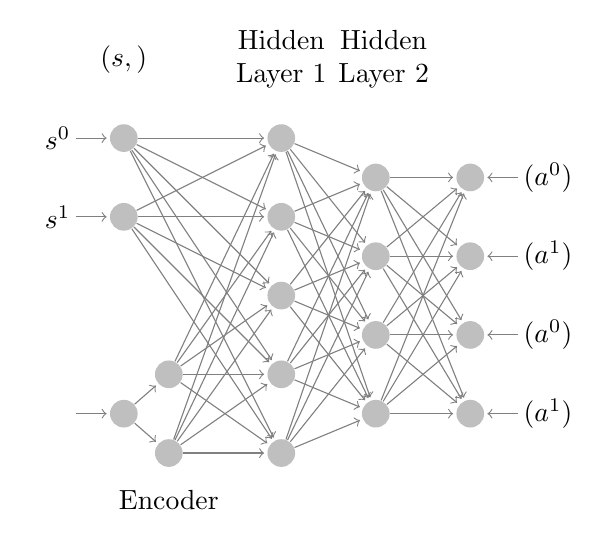
\begin{tikzpicture}[shorten >=1pt,->,draw=black!50, inner sep=1pt, node distance=\layersep]
        \tikzstyle{every pin edge}=[<-,shorten <=1pt]
        \tikzstyle{neuron}=[circle,fill=black!25,minimum size=10pt,inner sep=0pt]
        \tikzstyle{input neuron}=[neuron];
        \tikzstyle{input beta}=[neuron];
        \tikzstyle{qc}=[neuron];
        \tikzstyle{qr}=[neuron];
        \tikzstyle{hidden neuron}=[neuron];
        \tikzstyle{autoencoder neuron}=[neuron];
        \tikzstyle{annot} = [text width=4em, text centered]
        \tikzstyle{annot2} = [text width=10em, text centered]
        \def\layersep{2cm}
        % Draw the input layer nodes
        \foreach \name / \y in {0,...,1}
            \pgfmathtruncatemacro{\y}{0 + \y}
            \node[input neuron, pin=left:$s^\y$] (I-\name) at (0,-\y) {};

         % first layer
        \foreach \name / \y in {0,...,4}
        \pgfmathtruncatemacro{\y}{0 + \y}
            \path node[hidden neuron] (H1-\name) at (1*\layersep,-\y cm) {};

        \foreach \source in {0,...,1}
            \foreach \dest in {0,...,4}
                \path (I-\source) edge (H1-\dest);

        % BETA
        \node[input beta, pin=left:$\budgetaction$] (BETA) at (0,-3.5) {};

        % beta auto encoder
        \foreach \name / \y in {0,...,1}
            \pgfmathtruncatemacro{\ybis}{3+ \y}
            \path node[autoencoder neuron] (AE-\name) at (\layersep/3.5,-\ybis cm) {};



        \foreach \name / \y in {0,...,3}
        \pgfmathtruncatemacro{\y}{0 + \y}
            \path[yshift=-0.5cm]
            node[hidden neuron] (H2-\name) at (1.6*\layersep,-\y cm) {};


        % actions
        \foreach \name / \y in {0,...,1}
        \pgfmathtruncatemacro{\y}{0 + \y}
            \path[yshift=-0.5cm] node[qr,pin=right:$\Qr(a^\y)$] (Qr-\name) at (2.2*\layersep,-\y cm) {};

        \foreach \name / \y in {0,...,1}
        \pgfmathtruncatemacro{\yy}{2 + \y}
            \path[yshift=-0.5cm] node[qc,pin=right:$\Qc(a^\y)$] (Qc-\name) at (2.2*\layersep,-\yy cm) {};

        \foreach \source in {0,...,1}
            \foreach \dest in {0,...,4}
                \path (AE-\source) edge (H1-\dest);



        \foreach \dest in {0,...,1}
            \path (BETA) edge (AE-\dest);

         \foreach \source in {0,...,4}
            \foreach \dest in {0,...,3}
                \path (H1-\source) edge (H2-\dest);

        \foreach \source in {0,...,3}
            \foreach \dest in {0,...,1}
                \path (H2-\source) edge (Qr-\dest);

         \foreach \source in {0,...,3}
            \foreach \dest in {0,...,1}
                \path (H2-\source) edge (Qc-\dest);
        % Annotate the layers
       \node[annot] (input) at (0,1) {$(s,\budgetaction)$};
       \node[annot2] (input) at (\layersep/3.5,-4.6) {Encoder};
       \node[annot](h1) at (\layersep,1) {Hidden Layer 1};
       \node[annot](h2) at(1.65 * \layersep,1) {Hidden Layer 2};
       \node[annot](output) at(2.2* \layersep,1) {$\oQ$};
        %\node[annot,right of=hl] {Output layer};
    \end{tikzpicture}

    \caption[A Budgeted Fitted-$Q$ Neural-Network]{\acrlong{NN} for $\oQ$-functions approximation when $\cS=\Real^2$ and $|\cA| = 2$. Note that the current budget $\budget$ is not an input of the network as it has no influence on the returns.}
    \label{fig:architecture}
\end{figure}

\subsection{Parallel computing}
\label{subsec:parallel-computing}
In a simulated \idx{environment}, a first process that can be distributed is the collection of \idx{transition}s in the exploration procedure of \Cref{algo:risk-sensitive-exploration}, as $\budgetedpolicy_\text{greedy}$ stays constant within each minibatch\index{batch} which avoids the need of synchronisation between workers. Second, the main bottleneck of \gls{BFTQ} is the computation of the target $\abo \oQ$. Indeed, when computing $\budgetedpolicy_\text{hull}$ we must perform at each epoch a Graham-scan of complexity $\cO(|\cA||\tilde{\budgetspace}| \log |\cA||\tilde{\budgetspace}|)$ per \idx{transition} in $\cD$ to compute the convex hulls of $\oQ$ (where $\tilde{\budgetspace}$ is a finite discretisation of $\budgetspace$). The resulting total time-complexity is $\cO(\frac{|\cD||\cA||\tilde{\budgetspace}|}{1-\discountfactor} \log |\cA||\tilde{\budgetspace}|)$. This operation can easily be distributed over several CPUs provided that we first evaluate the \idx{model} $\oQ(\os',\cA \times \tilde{\budgetspace})$ for each state $\os$ extracted from the dataset $\cD$, which can be done in a single forward pass. By using multiprocessing in the computations of $\budgetedpolicy_\text{hull}$, we enjoy a linear speedup.
The full description of our scalable implementation of \gls{BFTQ} is recalled in \Cref{algo:bftq_full}.

\begin{algorithm}[tp]
\DontPrintSemicolon
\KwData{$\cD$, $\tilde{\budgetspace}$ a finite subset of $\budgetspace$, $\discountfactor$, a \idx{model} $\oQ\in (\Real^2)^{\ocS \times \ocA}$, a \idx{regression} algorithm \texttt{fit}, a set of \gls{CPU} workers $W$}
\KwResult{$\oQ^*$}
$\oQ \leftarrow 0$\;
$\overline{X} \leftarrow \{\os_{\indextransition},\oa_{\indextransition})\}_{{\indextransition}\in[0, |\cD|]}$\;
$\overline{S}' \leftarrow \{\os_{\indextransition}'\}_{{\indextransition}\in[0, |\cD|]}$\;
\Repeat{convergence}{
   Evaluate $\oQ(\overline{S}', \cA \times \tilde{\budgetspace})$ in a single forward pass\;
   Split $\cD$ among workers: $\cD = \cup_{w\in W} \cD_w$\;
   \For(\tcp*[f]{Run in parallel}){$w\in W$}{
       \For{$(\os_{\indextransition}=(\boldsymbol{\cdot},\budget_{\indextransition}),\oa_{\indextransition}=(\boldsymbol{\cdot},\budget_{a_{\indextransition}}),\overline{r}_{\indextransition} = ({r}_{\indextransition},{c}_{\indextransition}),\os_{\indextransition}'=(s'_{\indextransition},\boldsymbol{\cdot}) \in \cD$} {
           $\cP \leftarrow \{(\Qc(\os_i',\cA \times \tilde{\budgetspace}), \Qr(\os_i',\cA \times \tilde{\budgetspace}))\}$\;
           $\cP.\texttt{prune}()$ \tcp*[f]{Remove all dominated points}\;
           $\cH \leftarrow \texttt{convex\_hull}(\cP).\text{vertices}()$\tcp*[f]{in cw order}\;
           $k \leftarrow \min\{k: \budget_{\indextransition} \geq q_c$ with $\left(q_c,q_r\right) = \cH[k]\}$\;
           $q_c^2,q_r^2,q_c^1,q_r^1 \leftarrow \cH[k],\cH[k-1]$\;
           $p \leftarrow (\budget_{a_{\indextransition}} - q_a^1) / (q_c^2 - q_c^1)$\;
           $Y_c^{w,{\indextransition}} \leftarrow {c}_{\indextransition} + \discountfactor ((1-p) q_c^1+ p q_c^2)$\;
           $Y_r^{w,{\indextransition}} \leftarrow {r}_{\indextransition} + \discountfactor ((1-p) q_r^1+ p q_r^2)$\;
       }
   }
   Join the results: $\overline{Y} \leftarrow \cup_{w\in W} (Y_c^w, Y_r^w)$\;
   $\oQ \leftarrow \texttt{fit}(\overline{X}, \overline{Y})$\;
}
\caption{Scalable Budgeted Fitted-$Q$}
\label{algo:bftq_full}
\end{algorithm}

\section{Experiments}
\label{sec:experiements}
There are two hypotheses we want to validate.

\paragraph{Exploration strategies}\label{par:ex-explo} We claimed in \Cref{sec:exploration} that a \idx{risk-sensitive} exploration was required in the setting of \glspl{BMDP}. We test this hypotheses by confronting our strategy to a classical \idx{risk-neutral} strategy. The latter is chosen to be a \idx{$\egreedy$-greedy} \idx{policy} slowly transitioning from a random to a \idx{greedy} \idx{policy}\footnote{We train this \idx{greedy} policy using \gls{FTQ}.} that aims to maximise $\expectedvalue_{\policy} \return^{\policy}$ regardless of $\expectedvalue_{\policy} \constraintreturn^{\policy}$. The quality of the resulting batches\index{batch} $\cD$ is assessed by training a \gls{BFTQ} \idx{policy} and comparing the resulting performance.

\paragraph{Budgeted algorithms}\label{par:ex-brl} We compare our scalable \gls{BFTQ} algorithm described in \Cref{sec:scalable-bftq} to an \FTQl baseline. This baseline consists in approximating the \gls{BMDP} by a finite set of \glspl{CMDP} problems. We solve each of these \gls{CMDP} using the standard technique of \idx{Lagrangian Relaxation}: the cost constraint is converted to a soft penalty weighted by a Lagrangian multiplier $\lambda$ in a surrogate reward function: $\max_{\policy} \expectedvalue_{\policy}[\return^{\policy} - \lambda \constraintreturn^{\policy}]$. The resulting MDP can be solved by any RL algorithm, and we chose \gls{FTQ} for being closest to \gls{BFTQ}.
In our experiments, a single training of \gls{BFTQ} corresponds to 10 trainings of \FTQl policies. Each run was repeated $N_{\text{seeds}}$ times.

Parameters of the algorithms can be found in \Cref{sec:params:appendix}

\subsection{Environments}
\label{subsec:environments}
We evaluate our method on three different \idx{environment}s involving reward-cost trade-offs.

\paragraph{Corridors}
This simple \idx{environment} is only meant to highlight clearly the specificity of exploration in a budgeted setting. It is a continuous grid-world with Gaussian perturbations, consisting in a maze composed of two corridors: a risky one with high rewards and costs, and a safe one with low rewards and no cost. In both corridors the outermost cell is the one yielding the most reward, which motivates a deep exploration.

\begin{table}[ht!]
    \centering
    \begin{tabularx}{1.0\textwidth}{lll}
        \toprule
        Parameter & Description & Value\tabularnewline
        \midrule
        - & Size of the \idx{environment} & 7 x 6\tabularnewline
        - & \makecell[l]{Standard deviation of the Gaussian \\noise applied to actions} & (0.25,0.25)\tabularnewline
        H & Trajectory\index{trajectory} duration & 9\tabularnewline
        \bottomrule
    \end{tabularx}
    \caption{Parameters of \texttt{Corridors}}
    \label{tab:param-corridors}
\end{table}

\paragraph{Spoken Dialogue Systems}

Our second application is a dialogue-based\index{dialogue} \idx{slot-filling} simulation that has already benefited from \idx{batch} \gls{RL} optimisation in the past~\parencite{Lihong09,Chandramohan2010,pietquin2011sample}. As described in \Cref{sec:slot-filling-prob}, the system fills in a form of slot-values by interacting a \idx{user} through speech, before sending them a response. For example, in a restaurant reservation domain, it may ask for three slots: the area of the restaurant, the price-range and the food type. The \idx{user} could respectively provide those three slot-values: \texttt{Cambridge}, \texttt{Cheap} and \texttt{Indian-food}. In this application, we do not focus on how to extract such information from the \idx{user} utterances, we rather focus on decision-making for filling in the form. To that end, the system can choose among a set of generic actions. There are two ways of asking for a slot value: a slot value can be either be provided with an utterance, which may cause speech recognition errors\index{speech recognition error} with some probability, or by requiring the \idx{user} to fill-in the slots by using a numeric pad. In this case, there are no speech recognition errors\index{speech recognition error} but a counterpart risk of \idx{hangup}: we assume that manually filling a key-value form is time-consuming and annoying. The \idx{environment} yields a reward if all slots are filled without errors, and a constraint if the \idx{user} \idx{hangup}s. Thus, there is a clear trade-off between using utterances and potentially committing a mistake, or using the numeric pad and risking a premature \idx{hangup}.

\paragraph{Remark on the speech recognition\index{speech recognition}} As in \Cref{section:experiments-sigdial}, when receiving an utterance, the system can either understand it $(\mu=\mutop)$ or misunderstand it $(\mu=\mubot)$ with a fixed probability called the \gls{SER} $\ser$. Then, the \gls{SRS} is simulated: $\srs = (1+\exp(-x))^{-1}$ with $x\sim \normal(\mu, \sigma)$. It is the confidence score of the \gls{NLU} module about the last utterance. Note that here are no recognition errors ($\ser=0$ and $\srs=1$) when the \idx{user} provides information using the numeric pad.

\begin{table}[ht!]
    \centering
    \begin{tabularx}{1.0\textwidth}{lll}
        \toprule
        Parameter & Description & Value\tabularnewline
        \midrule
        $\ser$ & Sentence Error Rate & 0.6\tabularnewline
        $\mubot$& Gaussian mean for misunderstanding & -0.25\tabularnewline
        $\mutop$& Gaussian mean for understanding & 0.25\tabularnewline
        $\sigma$& Gaussian standard deviation & 0.6\tabularnewline
        $p$& Probability of \idx{hangup} & 0.25\tabularnewline
        H & Trajectory\index{trajectory} duration & 10\tabularnewline
        - & Number of slots & 3\tabularnewline
        \bottomrule
    \end{tabularx}
    \caption{Parameters of \texttt{Slot-Filling}}
    \label{tab:param-slot-filling}
\end{table}

\paragraph{Autonomous driving}
In our third application, we use the \href{https://github.com/eleurent/highway-env}{highway-env} \idx{environment} \parencite{Leurent2018} for simulated highway driving and behavioural decision-making.
We define a task that displays a clear trade-off between safety and efficiency. The \idx{agent} controls a vehicle with a finite set of manoeuvres implemented by low-lever controllers: $\mathcal{A}$ = \{\text{no-op}, \text{right-lane}, \text{left-lane}, \text{faster}, \text{slower}\}. It is driving on a two-lane road populated with other traffic participants: the vehicles in front of the \idx{agent} drive slowly, and there are incoming vehicles on the opposite lane. Their behaviours are randomised, which introduces some uncertainty with respect to their possible future trajectories\index{trajectory}.
The task consists in driving as fast as possible, which is \idx{model}led by a reward proportional to the velocity: $\reward(s_t, a_t) \propto v_t$. This motivates the \idx{agent} to try and overtake its preceding vehicles by driving fast on the opposite lane. This optimal but overly aggressive behaviour can be tempered through a cost function that embodies a safety objective: $\constraint(s_t, a_t)$ is set to $1/H$ whenever the ego-vehicle is driving on the opposite lane, where $H$ is the trajectory\index{trajectory} horizon. Thus, the constrained signal is the maximum proportion of time that the \idx{agent} is allowed to drive on the wrong side of the road.

\begin{table}[ht!]
    \centering
    \begin{tabularx}{1.0\textwidth}{lll}
        \toprule
        Parameter & Description & Value\tabularnewline
        \midrule
        $N_v$& Number of vehicles & 2 - 6\tabularnewline
        $\sigma_p$& Standard deviation of vehicles initial positions & 100 m\tabularnewline
        $\sigma_v$& Standard deviation of vehicles initial velocities & 3 m/s\tabularnewline
        H & Trajectory\index{trajectory} duration & 15 s\tabularnewline
        \bottomrule
    \end{tabularx}

    \caption{Parameters of \texttt{highway-env}}
    \label{tab:param-highway-env}
\end{table}

\subsection{Results}
\label{subsec:results}
In the following figures, each patch represents the mean and 95\% confidence interval over $N_{\text{seeds}}$ seeds of the means of $(\return^{\policy},\constraintreturn^{\policy})$ ($(\return^{\budgetedpolicy},\constraintreturn^{\budgetedpolicy})$ for \gls{BFTQ}) over $N_\text{trajs}$ trajectories\index{trajectory}. That way, we display the variation related to learning (and batches\index{batch}) rather than the variation in the execution of the policies.

We first bring to light the role of \idx{risk-sensitive} exploration in the \texttt{corridors} \idx{environment}: \Cref{fig:exploration} shows the set of trajectories\index{trajectory} collected by each exploration strategy, and the resulting performance of a \idx{budgeted policy} trained on each \idx{batch}. The trajectories\index{trajectory} (orange) in the \idx{risk-neutral} \idx{batch} are concentrated along the risky corridor (red) and ignore the safe corridor (green), which results in bad performances in the low-risk regime. Conversely, trajectories\index{trajectory} in the \idx{risk-sensitive} \idx{batch} (blue) are well distributed among both corridors and the corresponding \idx{budgeted policy} achieves good performance across the whole spectrum of risk budgets.

\begin{figure}[tp]
    \centering
    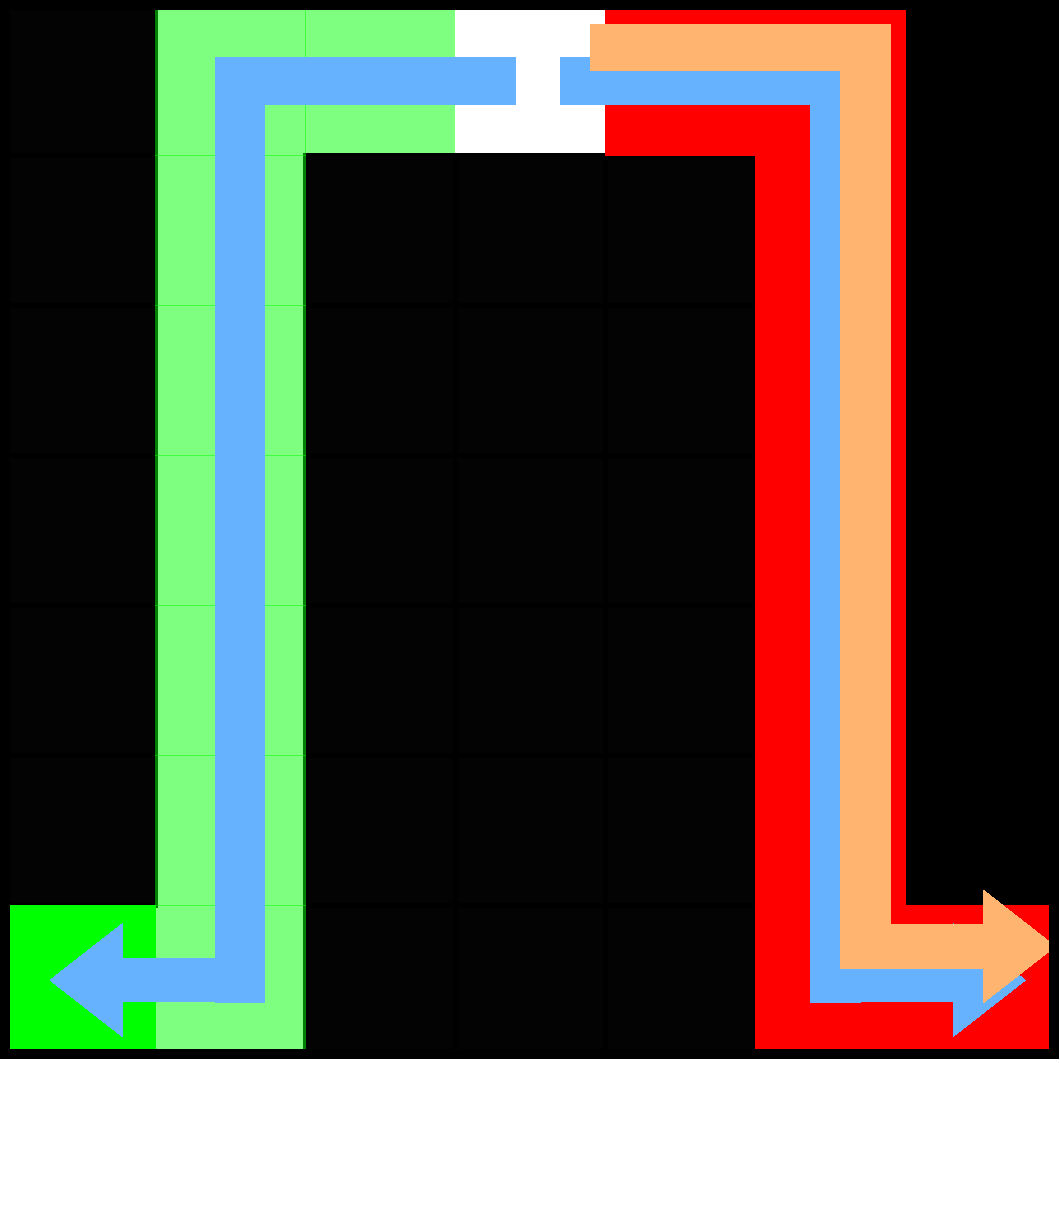
\includegraphics[width=0.4\textwidth]{sources/contribution/nips/source/img/test.pdf}\\
    %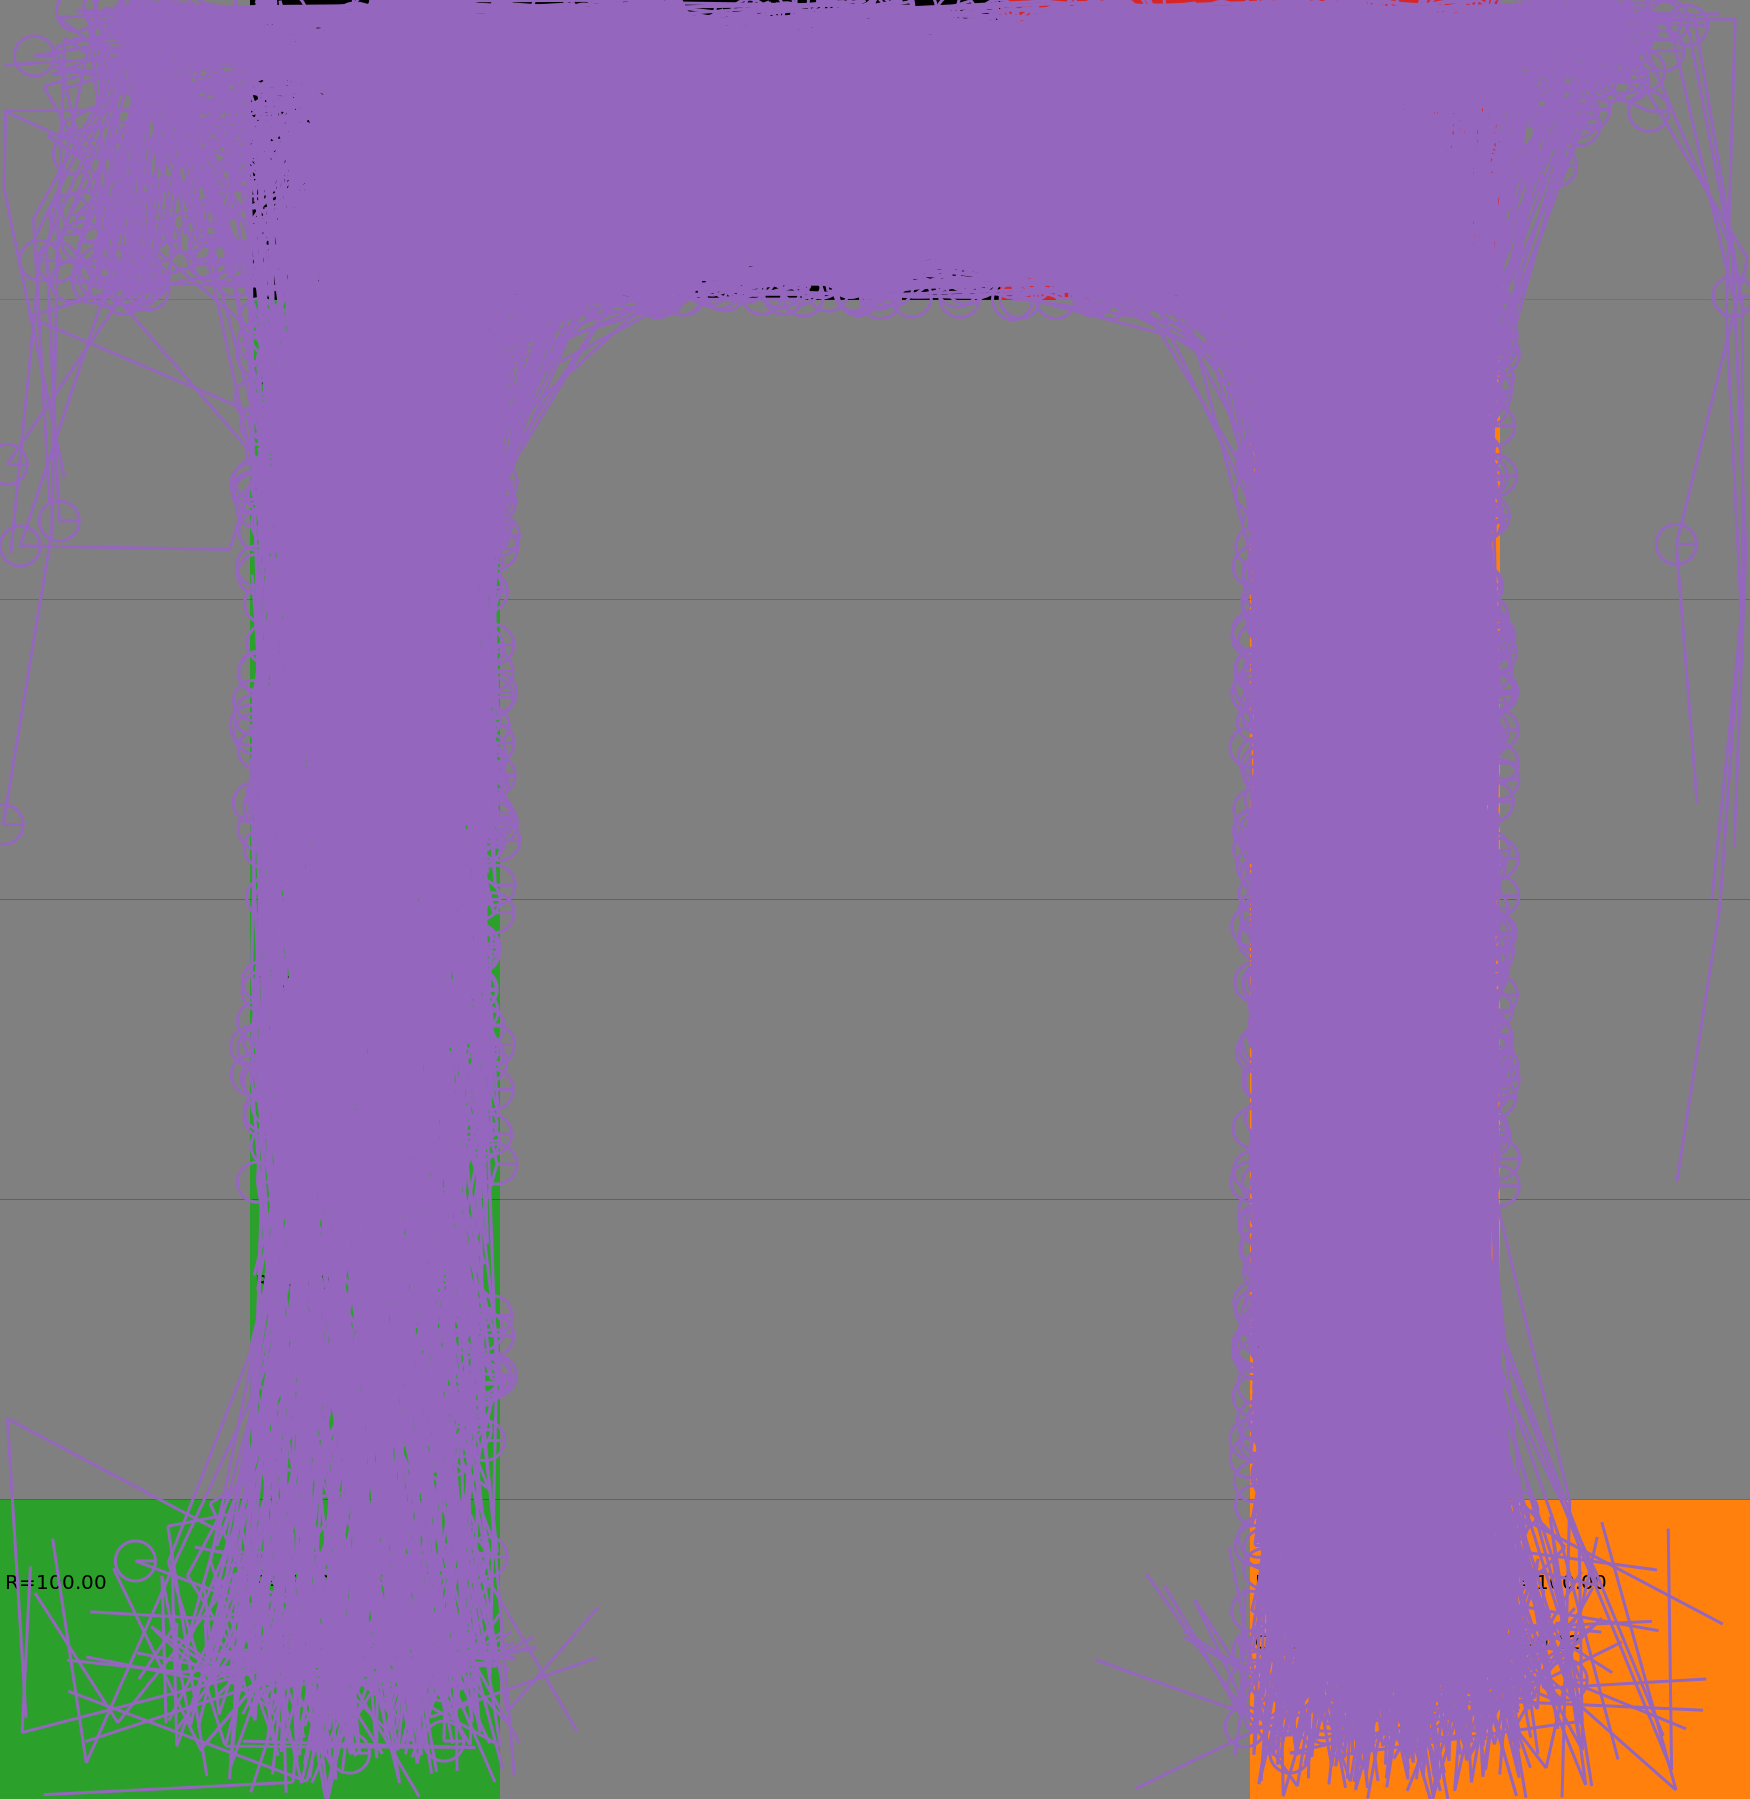
\includegraphics[width=0.23\textwidth]{source/img/risk-sensitive.png}
    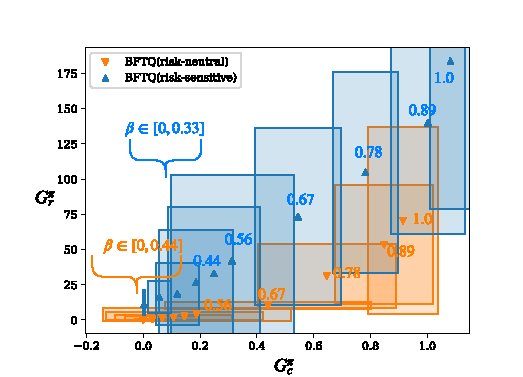
\includegraphics[page=1, width=0.75\textwidth]{sources/contribution/nips/source/img/corridors}
    \caption[Results on \texttt{Corridors}]{Trajectories (top) and performances (bottom) of two exploration strategies in the \texttt{corridors} \idx{environment}. }
    \label{fig:exploration}
\end{figure}


\begin{figure}[tp]
    \begin{center}
        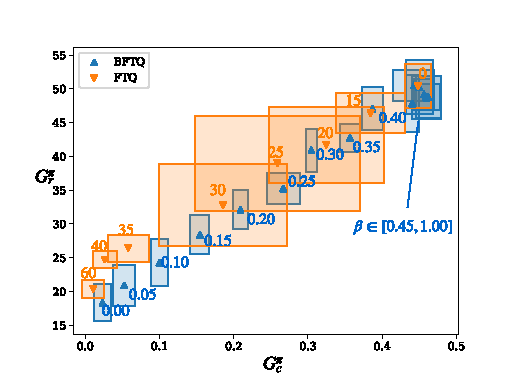
\includegraphics[width=0.75\linewidth]{sources/contribution/nips/source/img/slot-filling}\\
        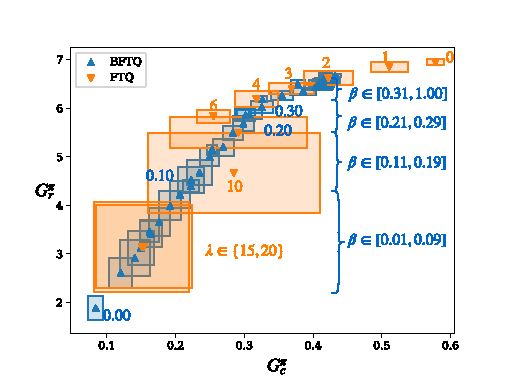
\includegraphics[width=0.75\linewidth]{sources/contribution/nips/source/img/highway}
        \caption[Results on \texttt{slot-filling} and \texttt{highway-env}]{Performance comparison of \FTQl and Budgeted Fitted-$Q$ on \texttt{slot-filling} (top) and \texttt{highway-env}(bottom) }
        \label{fig:results}
    \end{center}
\end{figure}

In a second experiment displayed in \Cref{fig:results}, we compare the performance of \FTQl to that of \gls{BFTQ} in the  \idx{dialogue} and autonomous driving tasks. For each algorithm, we plot the reward-cost trade-off curve. In both cases, \gls{BFTQ} performs almost as well as \FTQl despite only requiring a single \idx{model}. All budgets are well-respected on \texttt{slot-filling}, but on \texttt{highway-env} we can observe an underestimation of $\Qc$, since e.g. $\expectedvalue[\constraintreturn|\budget=0] \simeq 0.1 $. This underestimation can be a consequence of two approximations: the use of the sampling operator $\hat{\abo}$ instead of the true environmental operator $\abo$, and the use of the \gls{NN} function approximation $\oQ_{\params}$ instead of $\oQ$.
% This is probably due to \text{highway-env} being actually infeasible for $\budget=0$, since we noticed that about $8\%$ of bad initialisations occur with the front vehicle driving slower than the minimum velocity of the controlled vehicle, leading to either a front collision or a forced change to the opposite lane, both yielding costs.
Still, \gls{BFTQ} provides a better control on the expected cost of the policy, than \FTQl. In addition, \gls{BFTQ} behaves more consistently than \FTQl overall, as shown by its lower extra-seed variance.

\subsection{Budgeted Fitted-$Q$ policy executions}

In \Cref{table:dialogues}, we display two \idx{dialogue}s done with the same \gls{BFTQ} policy on \texttt{slot-filling}. The policy is given two budgets to respect in expectation, $\budget=0$ and $\budget=0.5$. For $\budget=0$, one can see that the system never uses the \texttt{ask\_num\_pad} action. Instead, it uses \texttt{ask\_oral} , an action subject to recognition errors. The system keeps asking for the same slot 2, because it has the lowest \gls{SRS}. It eventually summarises the form to the \idx{user}, but then reaches the maximum \idx{dialogue} length and thus faces a \idx{dialogue} failure. For $\budget=0.5$, the system first asks in a safe way, with \texttt{ask\_oral}. It may want to \texttt{ask\_num\_pad} if one of the \gls{SRS} is low. Then, the system proceeds to a confirmation of the slot values. If it is incorrect, the system continues the \idx{dialogue} using unsafe the \texttt{ask\_num\_pad} action to be certain of the slot values.

\begin{table}[tp]
    \centering
    \resizebox*{!}{\dimexpr\textheight-2\baselineskip\relax}{
    \begin{tabular}[]{lll}
        \toprule

        \idx{turn}&$\budget=0$&$\budget=0.5$\tabularnewline
        \midrule
        turn 0& \makecell[l]{valid slots: [0, 0, 0]\\ $\srs$: [ None None None ]\\ system says ASK\_ORAL(1) \\ user says INFORM} &\makecell[l]{ valid slots: [0, 0, 0]\\ $\srs$: [ None None None ]\\ system says ASK\_ORAL(2)\\ user says INFORM}\tabularnewline\midrule
        turn 1&\makecell[l]{valid slots: [0, 0, 0]\\ $\srs$: [ None 0.48 None ]\\ system says ASK\_ORAL(2) \\ user says INFORM} & \makecell[l]{valid slots: [0, 0, 1]\\ srs: [ None None 0.56 ]\\ system says ASK\_ORAL(0)\\ user says INFORM}\tabularnewline\midrule
        turn 2&\makecell[l]{valid slots: [0, 0, 0]\\ $\srs$: [ None 0.48 0.22 ]\\ system says ASK\_ORAL(0) \\ user says INFORM} & \makecell[l]{valid slots: [0, 0, 1] \\ srs: [ 0.30 None 0.56 ]\\ system says ASK\_ORAL(1)\\ user says INFORM}\tabularnewline\midrule
        turn 3&\makecell[l]{valid slots: [0, 0, 0]\\ $\srs$: [ 0.62 0.48 0.22 ]\\ system says ASK\_ORAL(2) \\ user says INFORM} & \makecell[l]{valid slots: [0, 0, 1]\\ srs: [ 0.30 0.54 0.56 ]\\ system says ASK\_ORAL(0)\\ user says INFORM}\tabularnewline\midrule
        turn 4&\makecell[l]{valid slots: [0, 0, 0] \\ $\srs$: [ 0.62 0.48 0.66 ]\\ system says ASK\_ORAL(1) \\ user says INFORM} & \makecell[l]{valid slots: [0, 0, 1]\\ srs: [ 0.68 0.54 0.56 ]\\ system says ASK\_NUM\_PAD(1)\\ user says INFORM}\tabularnewline\midrule
        turn 5&\makecell[l]{valid slots: [0, 1, 0]\\ $\srs$: [ 0.62 0.56 0.66 ]\\ system says ASK\_ORAL(2) \\ user says INFORM} & \makecell[l]{valid slots: [0, 1, 1]\\ $\srs$: [ 0.68 1.00 0.56 ]\\ system says SUMMARIZE\_AND\_INFORM\\ user says DENY\_SUMMARIZE}\tabularnewline\midrule
        turn 6&\makecell[l]{valid slots: [0, 1, 0]\\ $\srs$: [ 0.62 0.56 0.14 ]\\ system says ASK\_ORAL(2) \\ user says INFORM} & \makecell[l]{valid slots: [0, 1, 1]\\ $\srs$: [ 0.68 1.00 0.56 ]\\ system says ASK\_NUM\_PAD(2)\\ user says INFORM}\tabularnewline\midrule
        turn 7&\makecell[l]{valid slots: [0, 1, 1]\\ $\srs$: [ 0.62 0.56 0.30 ]\\ system says ASK\_ORAL(2) \\ user says INFORM }& \makecell[l]{valid slots: [0, 1, 1]\\ $\srs$: [ 0.68 1.00 1.00 ]\\ system says SUMMARIZE\_AND\_INFORM\\ user says DENY\_SUMMARIZE}\tabularnewline\midrule
        turn 8&\makecell[l]{valid slots: [0, 1, 1]\\ $\srs$: [ 0.62 0.56 0.49 ]\\ system says ASK\_ORAL(2) \\ user says INFORM} & \makecell[l]{valid slots: [0, 1, 1]\\ $\srs$: [ 0.68 1.00 1.00 ]\\ system says ASK\_NUM\_PAD(0)\\ user hangs up !}\tabularnewline\midrule
        turn 9&\makecell[l]{valid slots: [0, 1, 1]\\ $\srs$: [ 0.62 0.56 0.65 ]\\ system says SUMMARIZE\_AND\_INFORM \\ max size reached !}& \makecell[l]{ }\tabularnewline\bottomrule
    \end{tabular}
    }
    \caption[Example of Dialogue Policies executions]{Two dialogues generated by a safe policy ($\budget=0$) on the left and a risky one ($\budget=0.5$) on the right}
    \label{table:dialogues}
\end{table}

\section{Discussion}
\label{subsec:discussions}
\Cref{algo:bftq} is an algorithm for solving large unknown \glspl{BMDP} with continuous states. To the best of our knowledge, there is no algorithm in the current literature that combines all those features\index{feature}.

Algorithms have been proposed for \glspl{CMDP}, which are less flexible sub-problems of the more general \gls{BMDP}. When the \idx{environment} parameters ($\transition$, $\reward$, $\constraint$) are known but not tractable, solutions relying on function approximation~\parencite{Undurti} or approximate linear programming~\parencite{Poupart2015} have been proposed. For unknown \idx{environment}s, \idx{Online} algorithms \parencite{Geibel2005, Abe2010,AchiamHTA17,ChowGJP15} and a \idx{batch} algorithm \parencite{Thomas2015, Petrik2016, laroche2019,nadjahi2019safe,le2019batch} can solve large unknown \glspl{CMDP}. Nevertheless, these approaches are limited in that the constraints thresholds are fixed prior to training and cannot be updated in real-time at policy execution to select the desired level of risk.


\paragraph{Budgeted Markov Decision Processes algorithms}

To our knowledge, there were only two ways of solving a \gls{BMDP}. The first one is to approximate it with a finite set of \glspl{CMDP} (e.g. see our \FTQl baseline). As explained on \Cref{fig:Lagrangian}, the optimal \idx{deterministic policy} can be obtained by a line-search on the Lagrange multiplier values $\lambda$. Then, according to \textcite[Theorem 4.4]{BEUTLER1985236}, the optimal policy is a randomised mixture of two deterministic policies\index{deterministic policy}: the safest \idx{deterministic policy} that violates the constraint $\policy_{\lambda-}$ and the riskier of the feasible ones $\policy_{\lambda+}$. So \gls{FTQ} can be easily adapted for continuous states \gls{CMDP} and \gls{BMDP} through this methodology, but given the high variance it requires a lot of simulations to get a proper estimate of the calibration curve. Our solution not only requires one single \idx{model} but also avoids any supplementary interaction.

\begin{figure}[tp]
    \centering
    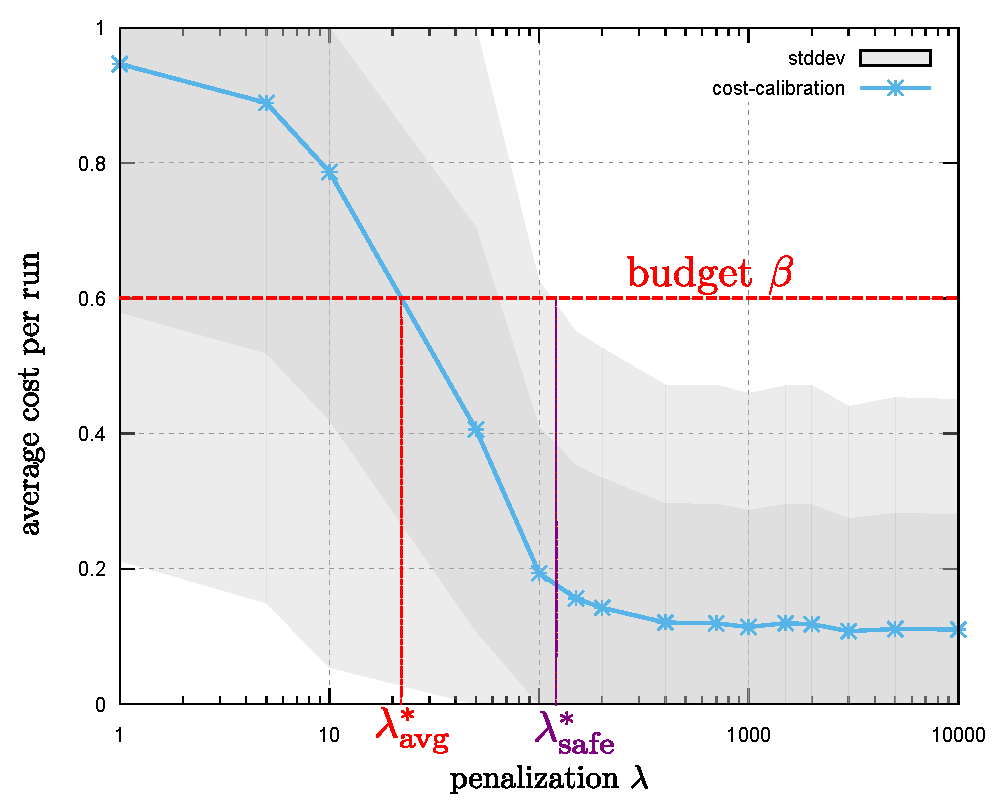
\includegraphics[width=0.75\textwidth]{sources/contribution/nips/source/img/CalibrationExample}
    \caption[Calibration for Lagragian Relaxation.]{Calibration of a penalty multiplier according to the budget $\budget$. The optimal multiplier $\lambda^*_{\text{avg}}$ is the smallest one to satisfy the budget constraint on average. Safer policies can also be selected according to the largest deviation from this mean cost.}
    \label{fig:Lagrangian}
\end{figure}


The only other existing \gls{BMDP} algorithm, and closest work to ours, is the \gls{DP} algorithm proposed by \textcite{Boutilier_Lu:uai16}. However, their work was established for finite state spaces only, and their solution relies heavily on this property. For instance, they enumerate and sort the next states $s'\in\cS$ by their expected value-by-cost, which could not be performed in a continuous state space $\cS$. Moreover, they rely on the knowledge of the \idx{model} ($\transition$, $\reward$, $\constraint$), and do not address the question of learning from interaction data.

\section{Conclusion}
\label{sec:conclusion}
The \gls{BMDP} framework is a principled framework for safe decision making under uncertainty, which could be beneficial to the diffusion of \gls{RL} in industrial applications, particularly dialogue systems. However, \glspl{BMDP} could so far only be solved in finite state spaces which limits their interest when dealing with continuous variable, as \gls{SRS} for example. We extend their definition to continuous states by introducing a novel \gls{DP} operator, that we build upon to propose a \gls{RL} algorithm. In order to scale to large problems, we provide an efficient implementation that exploits the structure of the value function and leverages tools from Distributed \gls{DRL}. We show that on two practical tasks, including a dialogue application, our solution performs similarly to a baseline \idx{Lagrangian relaxation} method while only requiring a single \idx{model} to train, and relying on an interpretable $\budget$ instead of the tedious tuning of the penalty $\lambda$. As a control is given over the hanging up frequency of an user, this framework makes a good candidate to design transferable\index{transfer} safe policies\index{safe policy} for \gls{DS} and this is the idea of the next chapter\footnote{Please note that we will use lagragian relaxation policies first to show if the idea of transferring safe policies actually works. As it won't work in our setting, we won't need to use BMDP policies.}.






